%!TEX root = ../../main.tex

\chapter{Entwurf}
In diesem Kapitel wird der Entwurf und die Architektur des Programms beschrieben. Zuerst wird beschrieben, welche Funktionen das Programm haben soll. Danach wird auf den Aufbau und die Architektur der Rest-API eingegangen. Es wird beschrieben, wie die Endpunkte der API gestaltet sind, welche Technologien verwendet werden und wie der innere Aufbau der API gestaltet ist.

% In diesem Kapitel wird auf die Struktur und Architektur der Rest-API eingegangen. Es wird zuerst beschrieben, wie die Endpunkte der API gestaltet sind und anschließend werden die verwendeten Technologien und der innere Aufbau beschrieben.

\section{Funktionen}
Das Programm soll eine Webanwendung sein auf der Nutzer mit einer benutzerfreundlichen Oberfläche verschiedene Eröffnungen betrachten und trainieren können. Es soll dabei als zentraler Ort dienen um Eröffnungen nachzuschauen und sein Gedächtnis aufzufrischen. Die Anwendung unterstützt Lernende, indem sie personalisiert Vorschläge macht, welche Eröffnung erneut abgefragt werden soll. Damit diese Anwendung umgesetzt werden kann sind die folgenden Funktionen notwendig.

\begin{itemize}
    \item Login: Ein Nutzer kann sich bei der Anwendung anmelden.
    \item Registrieren: Ein Nutzer kann sich einen Account anlegen.
    \item Spielumfang: Die Anwendung bietet zu Beginn jeweils eine Eröffnung für die weißen und für die schwarzen Figuren an.
    \item Lernmodus: Ein Nutzer kann eine Eröffnung auswählen und anschließend verschiedene Zugfolgen und Varianten der Eröffnung betrachten.
    \item Übungsmodus: Ein Nutzer kann eine Eröffnung auswählen und muss dann die Figuren einer Farbe nach der Zugfolge der Eröffnung bewegen. Der Computer spielt dabei die Züge des Gegners.
    \item Übungsmodus Hinweise: Während dem Üben hat ein Nutzer die Möglichkeit sich Hinweise geben zu lassen.
    \item Übungsmodus Erweiterung: Ein Nutzer hat die Möglichkeit nach einer Eröffnung die mit oder ohne Dekomposition das Spiel zu Ende zu spielen gegen einen Computergegner.
    \item Vorschläge: Ein Nutzer bekommt Vorschläge welche Eröffnung trainiert werden soll.
    \item Statistik: Ein Nutzer kann sich Statistiken zu den Eröffnungen anschauen. Dazu zählt die Anzahl an richtigen und falschen Übungsdurchläufen. Diese Statistik wird auch zur Erstellung der Vorschläge verwendet.
\end{itemize}

\section{Endpunkte}
Endpunkte in \ac{REST} sind ressourcenorientiert. Das bedeutet, die Pfade, die \ac{URI} genannt werden, bestehen aus einer hierarchischen Anordnung von Ressourcen. Die Funktion des Endpunkts wird über die HTTP-Methode beschrieben. Zum Beispiel wird durch GET eine Ressource angefragt, durch POST eine angelegt und durch DELETE wird sie gelöscht. Wenn eine Ressource eine Sammlung ist, wird der Endpunkt in der Mehrzahl notiert, auch dann, wenn nur auf ein einzelnes Element der Sammlung zugegriffen wird. Dadurch ist die Hierarchie einfacher zu erkennen. \todo{Quelle ergänzen}

In der hier entwickelten API gibt es die fünf Wurzelendpunkte \lstinline{/engine}, \lstinline{/login}, \lstinline{/openings}, \lstinline{/users} und \lstinline{/stats}. Diese spiegeln die verschiedenen Bestandteile des Backends wieder. Das besteht aus einer Schachengine, Authentifizierung, einem Eröffnungsbuch, Nutzerverwaltung und Statistiken.

Um die Kernfeatures der Anwendung zu ermöglichen werden die folgenden Endpunkte unter \lstinline{/openings} implementiert.

\begin{itemize}
    \item GET \verb|/openings|
    \item GET \verb|/openings/{id}/variants|
    \item GET \verb|/openings/{id}/variants/next-moves|
    \item GET \verb|/openings/{id}/next-move|
\end{itemize}

Mit ihnen kann man den Lern- und Übungsmodus umsetzen. Der Ablauf des Lernmodus ist in \autoref{fig:sd_opening_training} dargestellt. Er kann in den folgenden drei Schritten zusammengefasst werden.

\begin{enumerate}
     \item Der Nutzer wählt den Lernmodus aus. Das Frontend schickt eine GET Anfrage an den Endpuntk \lstinline{/openings}. Dieser liefert eine Liste von OpeningOverviews. Das sind JSON-Objekte, die die Namen und IDs der Wurzeleröffnungen darstellen. Die Namen werden dem Nutzer zur Auswahl gezeigt.
     \item Der Nutzer wählt die Eröffnung mit der ID D20 aus. Das Frontend schickt eine GET Anfrage an den Endpunkt \lstinline|/openings/D20/variants/next-moves|. Die API liefert die OpeningMoves zu allen Eröffnungen, die mit dem selben Namen anfangen den ersten Zug. OpeningMoves sind sind JSON-Objekte, die den Namen der Eröffnung und einen Zug im UCI-Format enthalten. Diese werden dem Nutzer angezeigt.
     \item Der Nutzer wählt aus, welchen Zug er ausführen möchte, zum Beispiel 1. d4. Das Frontend schickt eine GET Anfrage an \lstinline|/openings/D20/variants/next-moves?played=d2d4|. Diesmal werden die bereits ausgeführten Züge in dem Query-Parameter \lstinline{played} im UCI-Format übergeben. Die API liefert dann nur noch die Eröffnungen, die auch mit den selben Zügen anfangen. Dieser Schritt kann so oft wiederholt werden, bis keine weiteren Züge mehr vorhanden sind, also die Liste mit OpeningMoves leer ist.
\end{enumerate}

\begin{figure}
    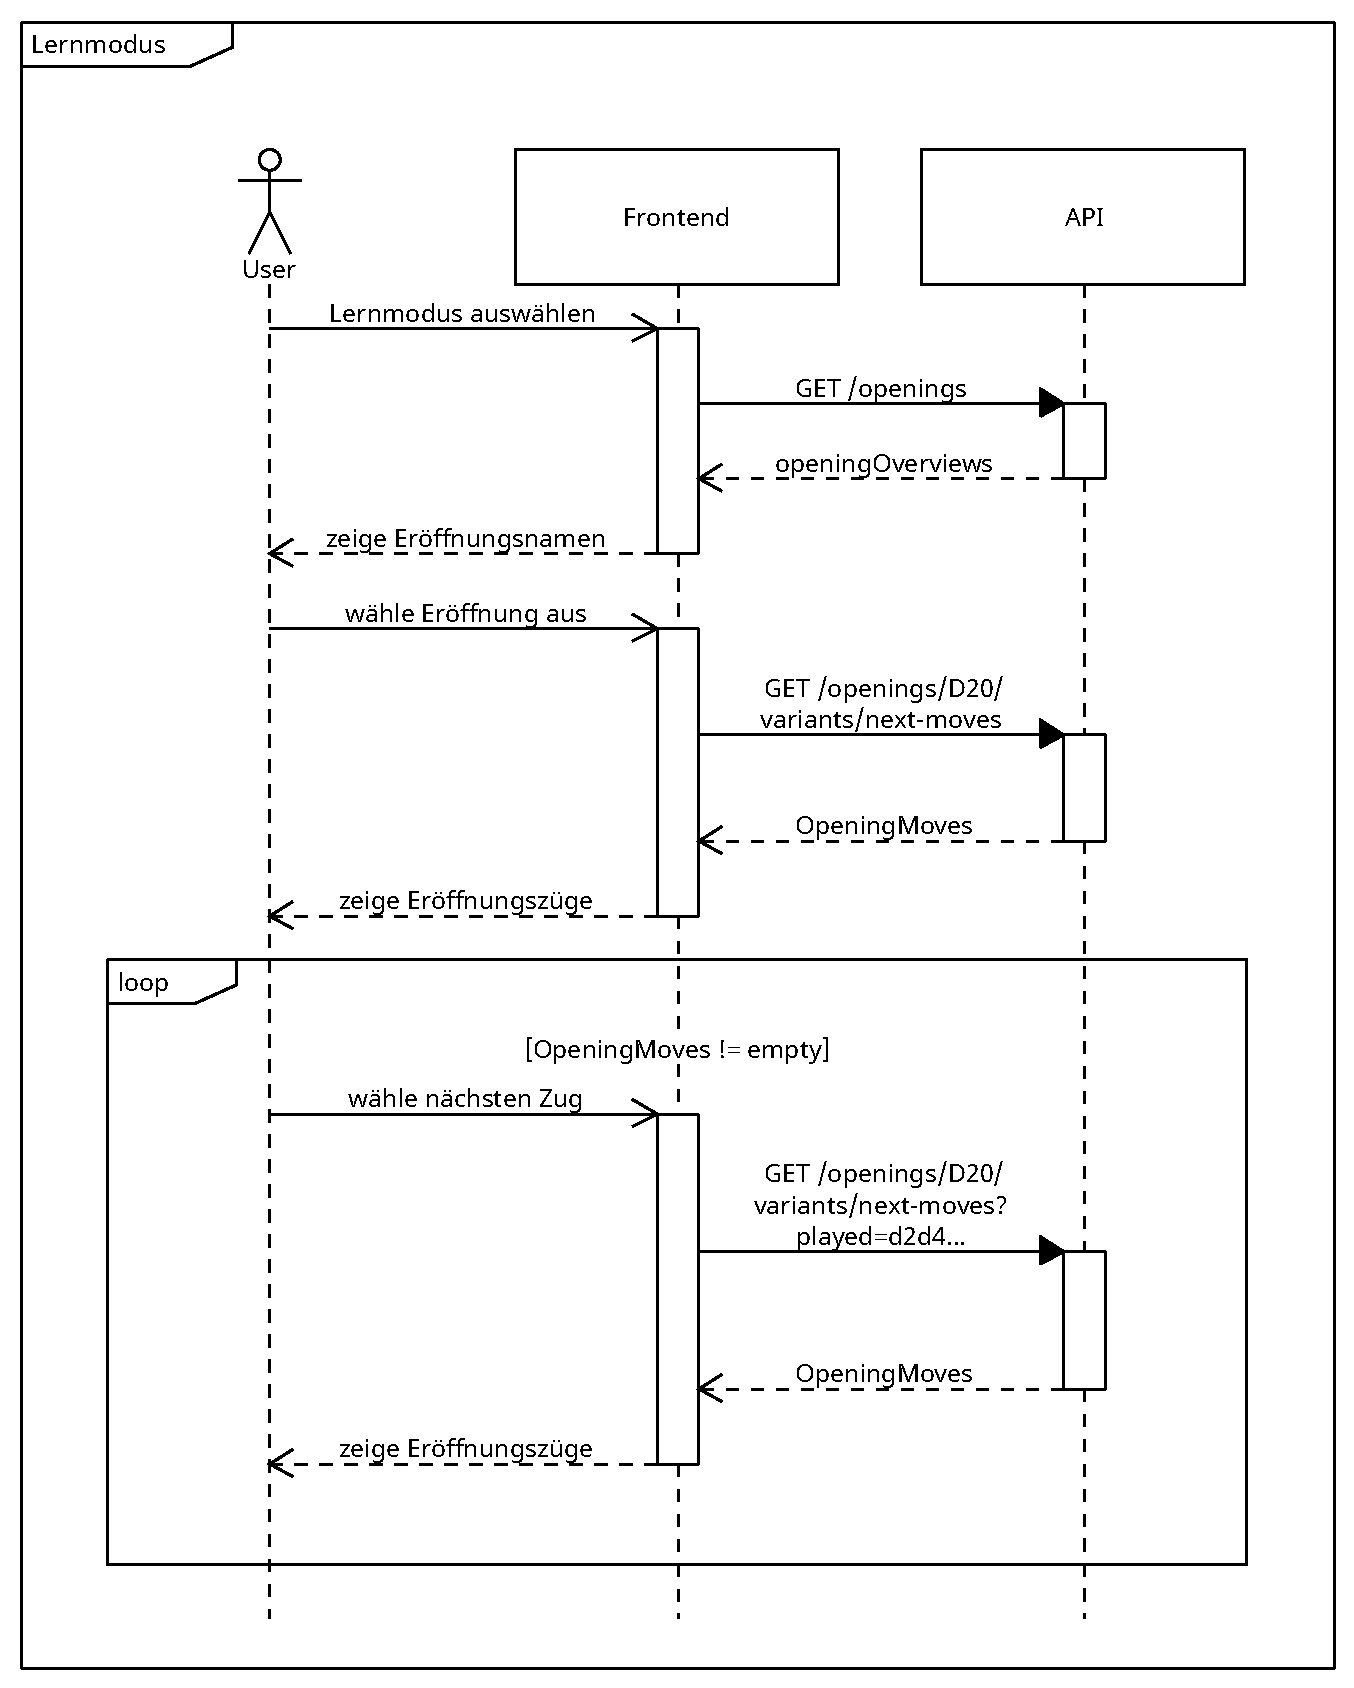
\includegraphics[width=\linewidth]{images/diagrams/sd_opening_training}
    \caption{Ablauf Übungsmodus}
    \label{fig:sd_opening_training}
\end{figure}

\section{Aufbau}
Als Programmiersprache wurde C\# gewählt aufgrund der guten Unterstützung und Dokumentation von Microsoft Bibliotheken. Außerdem kann C\# auf mehreren Plattformen ausgeführt werden und besitzt Typsicherheit durch statische Typisierung. Als Backend Framework wird .NET Core eingesetzt mit dem \ac{MVC} Pattern.
